\documentclass{article}

\usepackage{graphicx}          % Para graficos
\usepackage{hyperref}          % Para meter hipervinculos
\usepackage{soul}

\graphicspath{ {./informe/images/} }

\begin{document}

\begin{titlepage}
  \vspace*{1cm}

  \begin{center}
    {\Huge{Trabajo Práctico 1: Reliable File Transfer usnado UDP}}
  \end{center}

  \vspace{0.4cm}

  \begin{center}
    {\LARGE{Facultad de Ingeniería de la Universidad de Buenos Aires}}\\
    \vspace{0.3cm}
    {\Large{Redes}}\\
    \vspace{0.3cm}
    {\large{Cátedra Hamelin-Lopez Pecora}}\\
  \end{center}

  \vspace{0.8cm}
  \begin{center}
    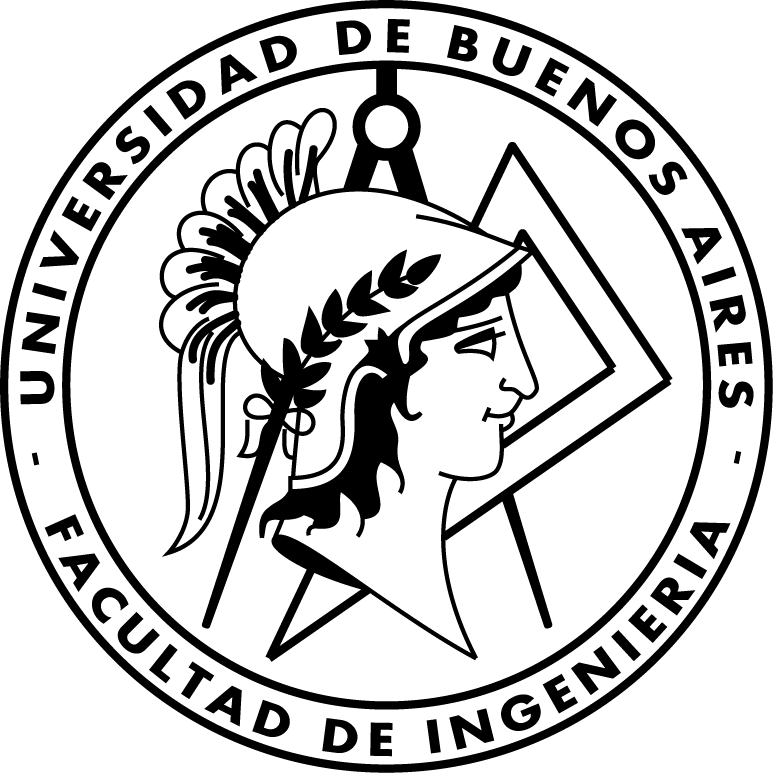
\includegraphics[scale=0.8]{Logo-fiuba}
  \end{center}

  \vspace{1.4cm}
  \begin{center}

    {\begin{minipage}{.5\textwidth}
        \begin{center}
          Demarchi, Ignacio\\
          {\small{Padrón: 107835}}\\
          {\small{email: PONER MAIl}}\\
        \end{center}
      \end{minipage}\begin{minipage}{.5\textwidth}
        \begin{center}
          Lijs, Theo\\
          {\small{Padrón: 109472}}\\
          {\small{email: PONER MAIL}}
        \end{center}
      \end{minipage}}

    \vspace{1.0cm}

    {\begin{minipage}{.5\textwidth}
        \begin{center}
          Schneider, Valentin\\
          {\small{Padrón: 107964}}\\
          {\small{email: PONER MAIL}}\\
        \end{center}
      \end{minipage}\begin{minipage}{.5\textwidth}
        \begin{center}
          Orsi, Tomas Fabrizio\\
          {\small{Padrón: 109735}}\\
          {\small{email: torsi@fi.uba.ar}}
        \end{center}
      \end{minipage}}

  \end{center}
\end{titlepage}

% \renewcommand*\contentsname{Indice}
\tableofcontents
\pagebreak

\section{\texorpdfstring{\textbf{Introducción}}{Introducción}}\label{introducciuxf3n}

El presente trabajo práctico tiene como objetivo la creación de una
aplicación de red. Para ello, se implemento un protocolo de aplicación
que corre sobre la capa de transporte utilizando UDP. El fin de este
protocolo es proveer un servicio de transferencia confiable de datos
(``Reliable Data Transfer''). Es decir, agregar un nivel de consistencia
en el envío de datos al protocolo de capa de transporte utilizado.

Para ello, se han implementado dos métodos de envío de datos. Stop \&
Wait y Selective Repeat. El protocolo entre cliente-servidor es
agnóstico a estos métodos, ya que solamente utiliza el socket que
proporciona Reliable Data Transfer y se abstrae de cómo funciona. El
socket de Reliable Data Transfer en sí es donde se puede optar por
enviar datos mediante Stop \& Wait o mediante Selective Repeat. Cada uno
con sus ventajas y desventajas. Leer las instrucciones proveídas en el
archivo ``README.md'' para cambiar de un modo a otro.

\section{\texorpdfstring{\textbf{Hipótesis y suposiciones realizadas
WIP}}{Hipótesis y suposiciones realizadas}}\label{hipuxf3tesis-y-suposiciones-realizadas-wip}

Antes de comenzar el TP creíamos que íbamos a poder diseñar un protocolo RDT utilizando un ``Socket RDT'' que por debajo utilizaba el socket UDP. Este iba a enviar y recibir la información de manera confiable para simplemente definir los mensajes a mandar del protocolo. De esta manera, el protocolo llamaría a este socket RDT y el socket se encargaría de mandar los mensajes del protocolo. Algo a tener en cuenta es que una suposición que se hizo fue que el protocolo es específico para el programa pedido en este trabajo práctico.

A su vez, debido a la arquitectura cliente y servidor, el socket debería ser capaz de establecer una conexión para garantizar la respuesta a múltiples peticiones de diferentes clientes por parte del servidor.

Por otro lado, con respecto a las metodologías de envío y recepción de paquetes: Selective Repeat y Stop and Wait, se asume que SR iba a ganarle en la mayoría de los casos a SW, debido a que SR implementa lo que se conoce como : pipelining.

\section{\texorpdfstring{\textbf{Implementación
WIP}}{Implementación}}\label{implementaciuxf3n-wip}

\subsection{Arquitectura Cliente-Servidor}\label{arquitectura-cliente-servidor}

La arquitectura Cliente-Servidor implementada es bastante estándar. El
servidor al iniciarse, queda a la escucha de nuevas conexiones.

Cuando el servidor logra recibir una request de conexión por parte de un
cliente; comienza el procedimiento de handshake. En este, el cliente le
envía al servidor la operación que quiere realizar (descarga o subida)
con el nombre del archivo correspondiente. El servidor contesta este
pedido de conexión con un el número del puerto con el cual el cliente
tiene que seguir la conversación. Cuando el cliente recibe dicho puerto,
envía un acknowledge final al servidor. Este comportamiento es
relativamente similar al concepto del ``welcoming socket'' en TCP.

Además de crear un nuevo socket para lidiar con el nuevo cliente, el
servidor también crea un nuevo thread para procesar el pedido
(``worker''). Esto se hace con el objetivo de que el servidor pueda
tratar con más de un cliente a la vez.

Una vez establecido el handshake, tanto el servidor como el cliente
comienzan a tratar con el envío y descarga de archivos. La manera en la
cual esta operación se lleva a cabo depende de la metodología usada
(``Selective Repeat'' o ``Stop and Wait'').

\subsection{SocketRDT}\label{socketrdt}

Toda la lógica relacionada a lograr el envío confiable de información
está encapsulada en la clase ``SocketRDT''. Esta es la que implementa
ambas metodologías, tanto de ``Selective Repeat'' como de ``Stop and
Wait''. Esta contiene los métodos ``send\_all()'' y ``receive\_all()'',
los cuales son los usados para el envío y recibimiento de archivos.

\subsection{Stop and Wait}\label{stop-and-wait}

En stop and wait, como indica su nombre, cada vez que el ``sender''
envía un paquete, espera hasta obtener su ack. Si, después de cierto
tiempo, no llega ningún tipo de respuesta, el sender asume que hubo
pérdida de paquete y vuelve a enviarlo.

El receiver, queda a la escucha del próximo paquete en la secuencia.
Cuando le llega dicho paquete, envía un paquete vacío con el mismo
sequence number del paquete que le llegó; esta es nuestra forma de hacer
un acknowledge.

\subsection{Selective Repeat}\label{selective-repeat}

En Selective Repeat, se introduce el concepto de la ventana. El sender
tiene una ventana de tamaño n; la cual representa todos los paquetes que
el sender va a verificar si tuvieron o no timeout. Este va a tratar de
enviar todos los paquetes de su ventana posibles, antes de comenzar a
escuchar por la llegada de acknowledges.

Si algún paquete tiene timeout, este paquete va a tomar prioridad sobre
el resto y va a ser enviado. En dicho caso, el sender va a vaciar el
buffer de recibidos del socket para ver todos los acknowledges
recibidos.

Además, en el caso de que se haya recibido el primer paquete de la
ventana, el sender va a actualizar la ventana. La nueva ventana va a
tener como nuevo comienzo el primer paquete sin ACK (esto hace provecho
del poder bufferear varios paquetes).

Por otro lado, el receptor va recibiendo paquetes y va enviando
acknowledges de cada paquete recibido. Para reconstruir el mensaje, usa
los sequence numbers de cada paquete.

\section{\texorpdfstring{\textbf{Pruebas}}{Pruebas}}\label{pruebas-wip}

\hl{(poner capturas de la terminal con lo que loguea el cliente y el
server) -\textgreater{} HACER PRETTY PRINT ANTES DE ESTO}

\textbf{Sin perdida}

Alquimista 5MB stop \& wait

Alquimista 5MB selective repeat

Grupo12 1MB stop \& wait

Grupo12 1MB selective repeat

\textbf{Perdida 10\%}

Rick 5MB stop \& wait

Rick 5MB selective repeat

Grupo12 1MB stop \& wait

Grupo12 1MB selective repeat

\textbf{Perdida 50\%}

Rick 5MB stop \& wait

Rick 5MB selective repeat

Grupo12 1MB stop \& wait

Grupo12 1MB selective repeat

\section{\texorpdfstring{\textbf{Mininet}}{Mininet}}\label{mininet}

La topología utilizada para el trabajo práctico es la siguiente:

\begin{center}
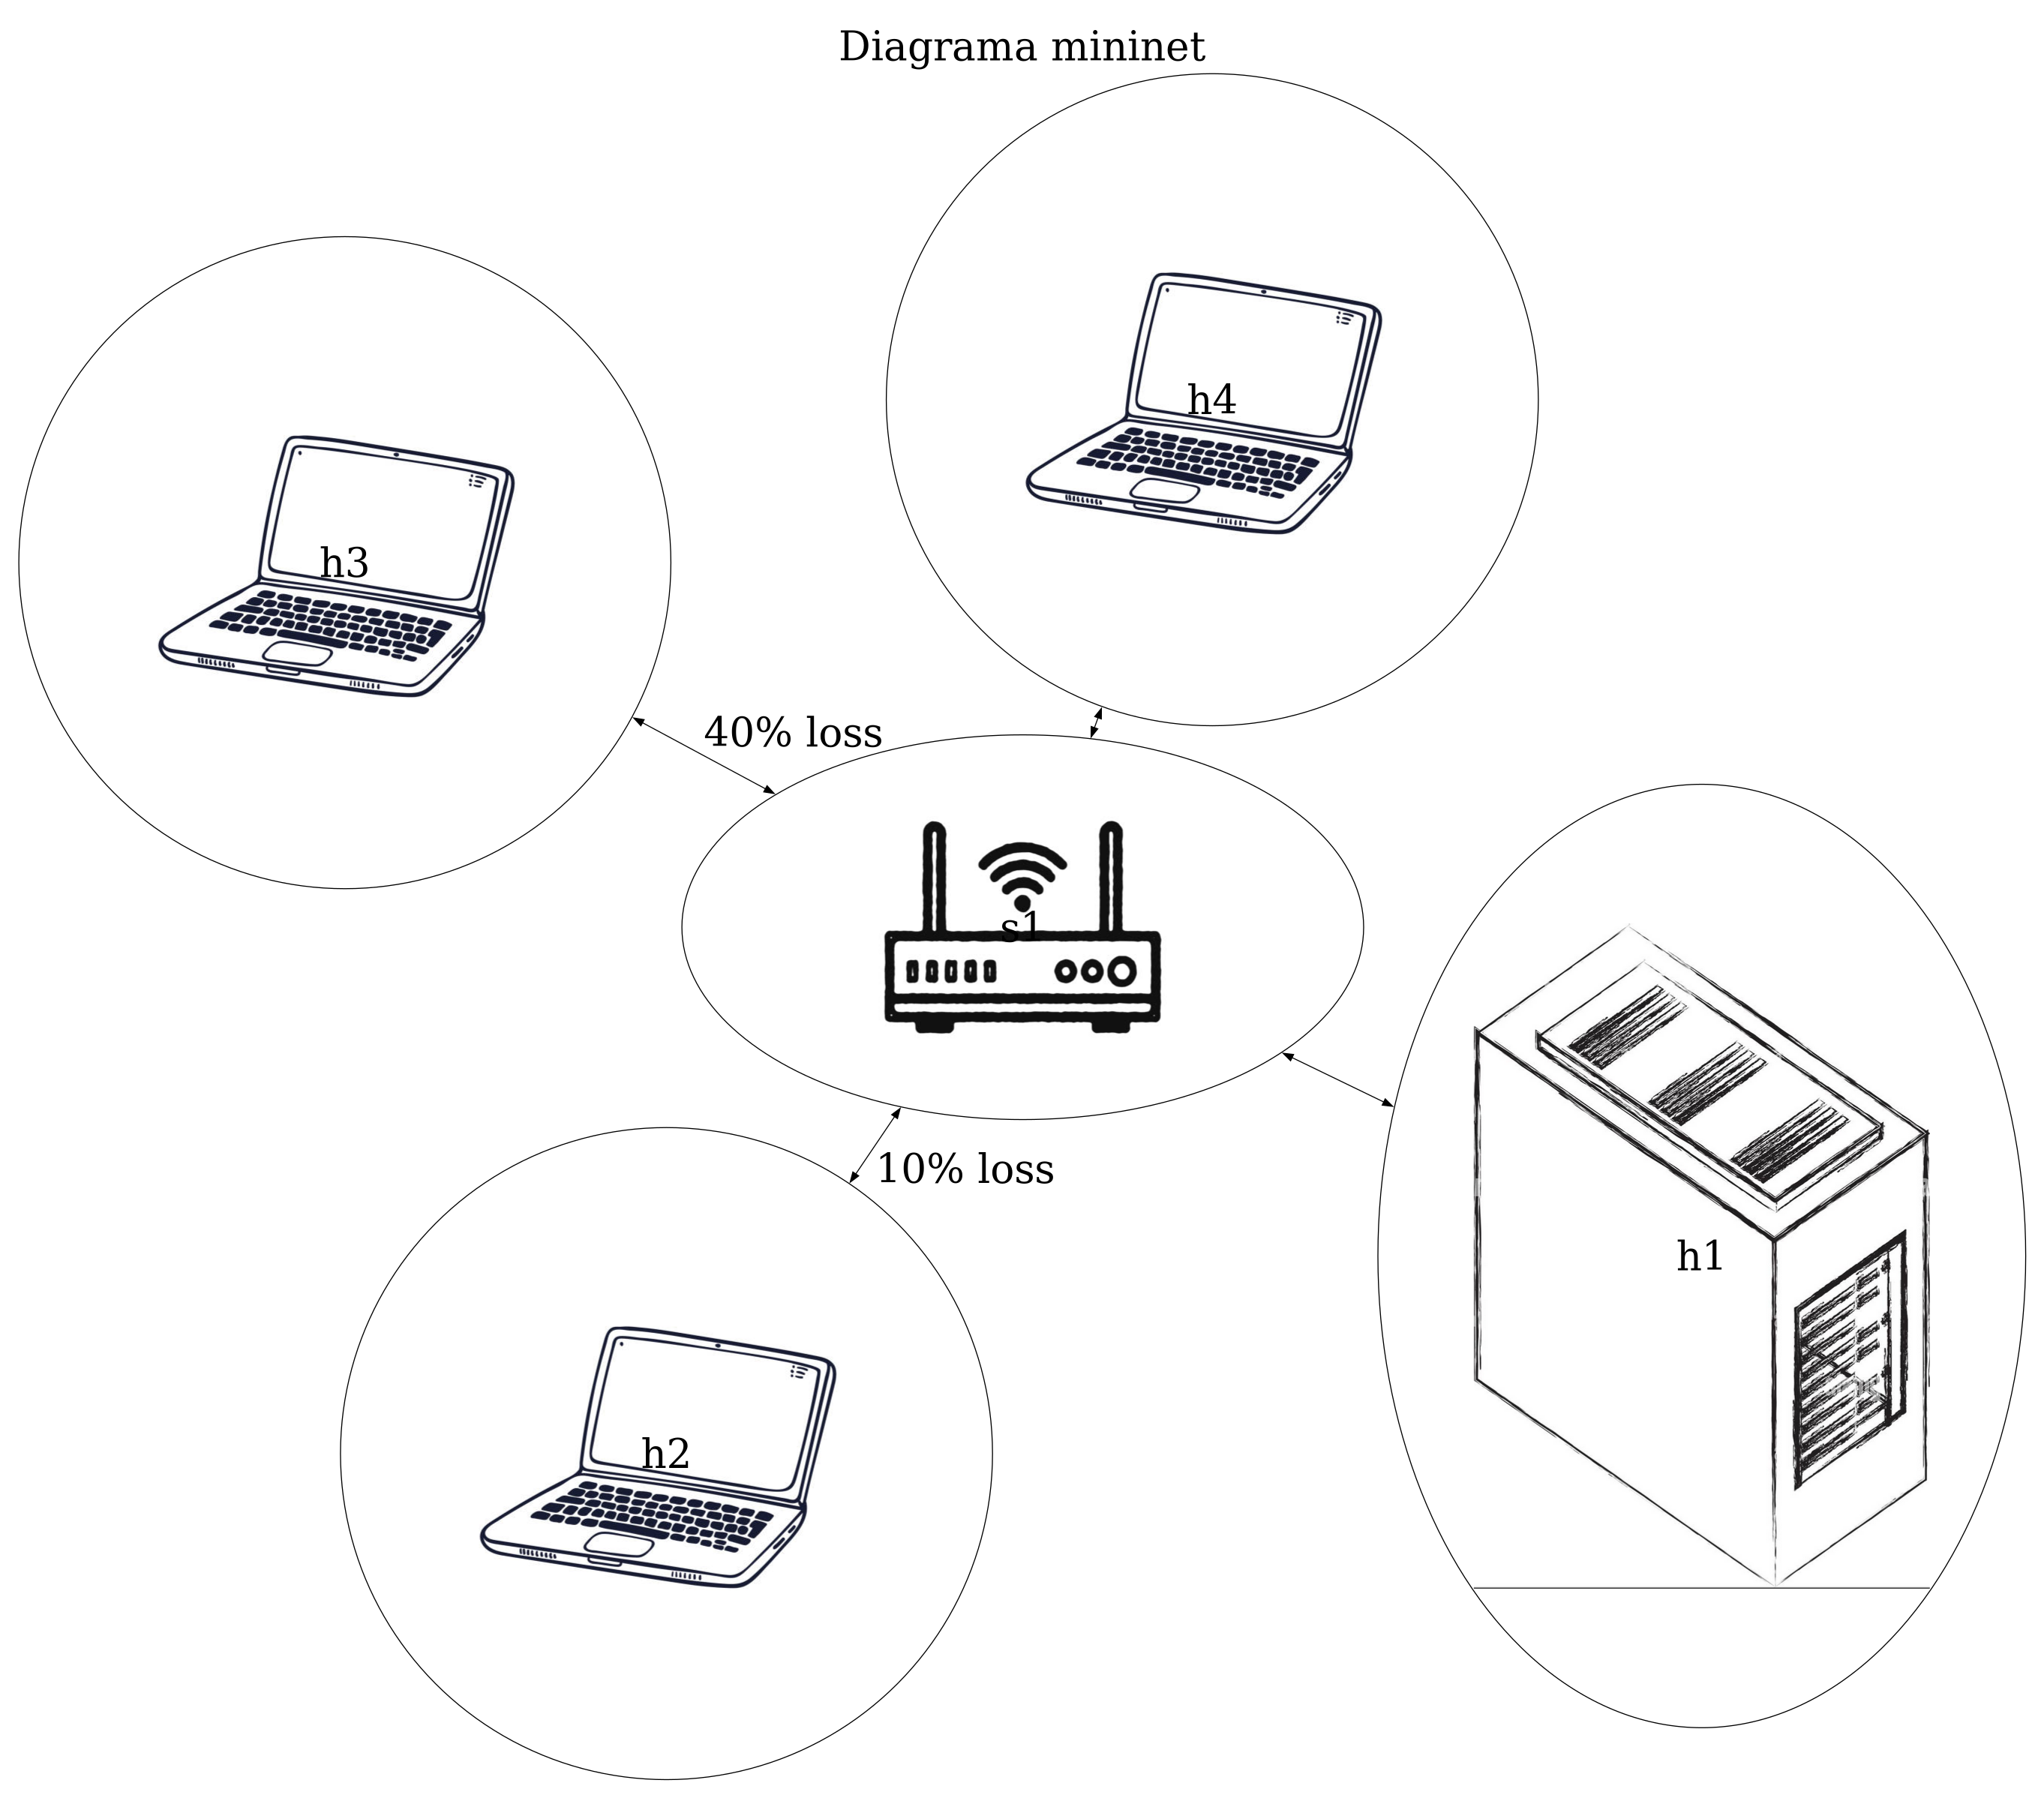
\includegraphics[scale=0.09999999999]{diagramaMininet}
\end{center}

Donde, por convención, decidimos correr el servidor en h1, pero
realmente se puede desde cualquier host, siempre y cuando se seteen las
IPs correctamente.

La topología la tenemos establecida con un archivo ``.py'' para poder
tenerla configurada fácilmente. La misma consta de 4 hosts conectados a
un único switch, con el host h2 y h3 seteados para tener pérdida de
paquetes.

\section{\texorpdfstring{\textbf{Preguntas a responder}}{Preguntas a responder}}\label{preguntas-a-responder}

\subsection{\texorpdfstring{\textbf{1. Describa la arquitectura Cliente-Servidor.}}{1. Describa la arquitectura Cliente-Servidor.}}\label{describa-la-arquitectura-cliente-servidor.}

En la arquitectura cliente-servidor siempre hay un host activo, llamado servidor, quien atiende las solicitudes de muchos otros hosts, denominados clientes. Los clientes no se comunican directamente entre sí, si no con el servidor. Otra característica de esta arquitectura es que el servidor mantiene una IP fija y conocida, para que los clientes puedan establecer conexiones cuando lo deseen, enviando peticiones a esa IP.

\textbf{2. ¿Cuál es la función de un protocolo de capa de aplicación?}

La función principal de un protocolo de capa de aplicación es establecer
reglas para la comunicación entre aplicaciones que se encuentran en 2
hosts diferentes.

Una de las principales funciones de las que deben encargarse los
protocolos a nivel capa de aplicación, es que dos aplicaciones corriendo
en 2 procesos diferentes puedan entenderse entre sí.

Una consecuencia directa del modelo de capas es que las aplicaciones
pueden abstraerse de estar corriendo en hosts separados por kilómetros
de distancia ya que simplemente relegan el envío y recibo de datos a la
capa de transporte, que apoyándose en las capas siguientes, se encargan
de que los datos se transmitan entre host y host.

\subsection{\texorpdfstring{\textbf{3. Detalle el protocolo de
aplicación desarrollado en este trabajo.}}{3. Detalle el protocolo de aplicación desarrollado en este trabajo.}}\label{detalle-el-protocolo-de-aplicaciuxf3n-desarrollado-en-este-trabajo.}

Nuestro protocolo de aplicación es una wrapper fino para nuestra implementación de Socket. No hay procesamiento adicional a los archivos, más allá de transformarlos a tiras de bytes.

A nivel mensaje, cada archivo se parte en varios paquetes. Cada paquete tiene como peso máximo 512 bytes. 8 de esos bytes están dedicados al header.

\hl{El header tiene:}

\begin{itemize}
\item
  Sequence number (4 bytes)
\item
  Flag de conexión
\item
  Flag de tipo de conexión
\item
  Flag de fin de conexión
\item
  Flag de error
\end{itemize}

Los otros 504 bytes son dedicados al payload.

Durante el handshake, la flag de conexión está encendida y el cliente indica el tipo de conexión. Cuando comienza el envío de información la flag de conexión se pone en 0.

Cuando la información termina, se enciende la flag de FIN.

En caso de que haya un error en la comunicación, se enciende la flag de error y la comunicación se cierra.

\subsection{\texorpdfstring{\textbf{4. La capa de transporte del stack
TCP/IP ofrece dos protocolos: TCP y UDP. ¿Qué servicios proveen dichos
protocolos? ¿Cuáles son sus características? ¿Cuándo es apropiado
utilizar cada
uno?}}{4. La capa de transporte del stack TCP/IP ofrece dos protocolos: TCP y UDP. ¿Qué servicios proveen dichos protocolos? ¿Cuáles son sus características? ¿Cuándo es apropiado utilizar cada uno?}}\label{la-capa-de-transporte-del-stack-tcpip-ofrece-dos-protocolos-tcp-y-udp.-quuxe9-servicios-proveen-dichos-protocolos-cuuxe1les-son-sus-caracteruxedsticas-cuuxe1ndo-es-apropiado-utilizar-cada-uno}

TCP:

\begin{itemize}
\item
  \textbf{Confiabilidad}: garantiza la entrega de datos, en orden, y sin
  errores.
\end{itemize}

\begin{itemize}
\item
  \textbf{Control de flujo}: regula la velocidad de transmisión de datos
  para evitar la congestión en el end-host.
\item
  \textbf{Control de congestión}: regula la velocidad de transmisión de
  datos para evitar la congestión en la red.
\item
  \textbf{Orientado a la conexión}: establece una conexión entre el
  emisor y el receptor antes de la transferencia de datos, para poder
  negociar los parámetros de la misma.
\item
  Tiene \textbf{mayor complejidad} que UDP debido a la gestión de la
  conexión, por lo que tiene una demora significativa para enviar y
  recibir información. Por esto, conviene utilizar TCP cuando se
  necesite una transmisión de datos confiable, por sobre la transmisión
  rápida.
\end{itemize}

UDP:

\begin{itemize}
\item
  \textbf{No hay confiabilidad:} no se garantiza la entrega de datos, ni
  el orden en que lleguen
\item
  \textbf{Envío de datos sin conexión}: no se establece una conexión
  antes de enviar datos, el cliente directamente le envia paquetes al
  server, (que pueden llegar o no) y el servidor puede contestar o no.
\item
  Tiene una \textbf{menor complejidad} que TCP, ya que tiene menor
  cantidad de tareas que procesar. Además, al no preocupar se por
  garantizar la entrega de datos confiable, se consigue una mejor
  latencia que TCP.
\item
  Justamente por el punto anterior, UDP conviene cuando se necesita
  priorizar una entrega rápida, pero no necesariamente de toda la
  información completa, como por ejemplo una videollamada, o juegos
  online.
\end{itemize}

\section{\texorpdfstring{\textbf{Dificultades
encontradas}}{Dificultades encontradas}}\label{dificultades-encontradas}

Una de las principales dificultades que encontramos fue lograr que el
handshake fuese reliable. Una vez ``pasada la barrera del handshake'',
el protocolo funcionaba sin muchos problemas (incluso con pérdida).

Para solucionar esto, tuvimos que asegurarnos de que cada uno de los
mensajes del handshake (syn, synack, ack) llegasen de forma reliable.

Otro problema del handshake, es que no se podía crear el socket en el
puerto antes de terminar el handshake. Esto se debía a que, si se perdía
el paquete de synack, el cliente no iba a poder saber el nuevo puerto
con el que tiene que hablar e iba a saltar timeout. La resolución de
esto fue tratar el handshake en el puerto del servidor.

\section{\texorpdfstring{\textbf{Conclusión
WIP}}{Conclusión}}\label{conclusiuxf3n-wip}

A la hora de enviar archivos nos topamos con el límite de tamaño de 4GB debido a que para enviar un int hicimos uso de htonl, la cual manda hasta un long de uint32.



Basándonos en la bibliografía, suponíamos que la metodología ``Selective Repeat'' iba a ser más eficiente que ``Stop and Wait''. Ya que ``Stop and Wait'' no hacía provecho de un buffer para almacenar paquetes fuera de orden.

Sin embargo, resultó que el tamaño de la ventana en ``Selective Repeat'' es un factor que influye bastante en la eficiencia del mismo. Y que incluso, dado una ventana muy grande y timeouts muy cortos;siempre ``Selective Repeat'' puede terminar siendo menos eficiente que ``Stop and Wait''.

\end{document}